\documentclass[11pt]{article}

% ---------- Packages ----------
\usepackage[a4paper, margin=2.4cm]{geometry}
\usepackage[utf8]{inputenc}
\usepackage[T1]{fontenc}
\usepackage{lmodern}
\usepackage[english]{babel}
\usepackage{xcolor}
\usepackage{titlesec}
\usepackage{enumitem}
\usepackage{fancyhdr}
\usepackage{hyperref}
\usepackage{tikz}
\usetikzlibrary{positioning, arrows.meta, fit, backgrounds, shapes.misc}
\usepackage{tcolorbox}
\tcbuselibrary{skins, breakable}

% ---------- Colors ----------
\definecolor{inkNavy}{HTML}{1B2A4A}
\definecolor{accentTeal}{HTML}{0E7C7B}
\definecolor{accentAmber}{HTML}{C97A2C}
\definecolor{softGray}{HTML}{6B7280}
\definecolor{bgPlanner}{HTML}{EAF3F3}
\definecolor{bgBuild}{HTML}{FBF1E6}
\definecolor{bgAudit}{HTML}{EEF0F8}
\definecolor{lineGray}{HTML}{D7DBE0}

% ---------- Heading typography ----------
\titleformat{\section}
  {\Large\bfseries\color{inkNavy}}
  {\thesection}{0.5em}{}
\titlespacing*{\section}{0pt}{1.4em}{0.8em}

\titleformat{\subsection}
  {\large\bfseries\color{accentTeal}}
  {\thesubsection}{0.5em}{}
\titlespacing*{\subsection}{0pt}{1.1em}{0.5em}

% ---------- Header/footer ----------
\pagestyle{fancy}
\fancyhf{}
\renewcommand{\headrulewidth}{0pt}
\fancyfoot[L]{\small\color{softGray}\href{https://github.com/dramirezbe/SelfHostedContextCrafter}{SelfHostedContextCrafter} --- Concept document}
\fancyfoot[R]{\small\color{softGray}\thepage}

\hypersetup{
  colorlinks=true,
  linkcolor=accentTeal,
  urlcolor=accentTeal,
  pdftitle={SelfHostedContextCrafter},
  pdfauthor={SelfHostedContextCrafter},
  pdfsubject={Self-hosted agent orchestrator for scoped planning and code auditing}
}

\setlist[itemize]{leftmargin=1.4em, itemsep=0.3em, topsep=0.3em}

% Reusable concept box
\newtcolorbox{ideabox}[1]{
  enhanced, breakable,
  colback=white, colframe=lineGray,
  boxrule=0.5pt, left=10pt, right=10pt, top=8pt, bottom=8pt,
  borderline west={2.5pt}{0pt}{accentTeal},
  before upper={\textbf{\color{inkNavy}#1}\\[4pt]}
}

\begin{document}

% ================= COVER PAGE =================
\begin{titlepage}
\centering
\vspace*{2.2cm}

{\color{softGray}\large SELF-HOSTED AGENT ORCHESTRATOR}\\[0.6cm]

{\Huge\bfseries\color{inkNavy} \href{https://github.com/dramirezbe/SelfHostedContextCrafter}{SelfHostedContextCrafter}}\\[0.5cm]

{\Large\color{accentTeal} Scoped planning and code auditing\\ on local infrastructure}

\vspace{1.8cm}


\begin{tikzpicture}
\draw[accentAmber, line width=1.2pt] (-3,0) -- (3,0);
\end{tikzpicture}

\vspace{1.8cm}

{\large\color{softGray} Concept document --- Idea proposal}

\vspace{0.4cm}

{\color{softGray} \today}

\vfill

{\small\color{softGray} A system that separates \emph{thinking} (planning with verifiable context),\\ \emph{doing} (building with a human in control), and \emph{verifying} (auditing against the source),\\ all running on your own hardware.}

\end{titlepage}

% ================= EXECUTIVE SUMMARY =================
\section*{Executive summary}
\addcontentsline{toc}{section}{Executive summary}

\href{https://github.com/dramirezbe/SelfHostedContextCrafter}{SelfHostedContextCrafter} is a \textbf{self-hosted} LLM agent orchestrator designed for teams developing software under real-world constraints --- specific hardware, business requirements, and regulations --- who cannot (or do not want to) send that information to a cloud AI provider.

The core idea is simple but uncommon among today's tools: \textbf{the agent never writes production code}. Its only job is to read and digest all relevant technical documentation (hardware datasheets, requirements, regulations, architecture context) and produce a scoped, traceable \emph{advanced plan}. That plan is what a human --- supported by their own code agent --- uses to build. Once the code exists, a second mode of the same system \textbf{audits} it against the plan and the original documentation, returning a per-module score, suggested changes, and specific warnings.

The entire cycle runs on local hardware, with self-hosted LLM models, which makes this approach viable in contexts where the confidentiality of hardware, code, or regulations is a requirement, not a preference.

% ================= THE PROBLEM =================
\section{The problem}

Current code assistants are powerful at generating text, but they share three recurring weaknesses in projects with real-world constraints:

\begin{itemize}
  \item \textbf{They lose the original context.} They generate reasonable-looking code in the moment, but without clear traceability back to the requirement, regulation, or hardware datasheet that originated it.
  \item \textbf{They hallucinate when context is scattered.} The more fragmented the documentation (manufacturer PDFs, regulations, internal specs), the easier it is for the model to fill gaps with assumptions.
  \item \textbf{They require sending sensitive information to external services.} Proprietary hardware, internal regulations, or source code cannot always leave the organization.
\end{itemize}

On top of this there is a \textbf{control} problem: when an agent generates and audits its own code in the same step, there is no real independent verification --- it is the same reasoning reviewing itself.

% ================= THE CORE IDEA =================
\section{The core idea}

\href{https://github.com/dramirezbe/SelfHostedContextCrafter}{SelfHostedContextCrafter} splits the development cycle into three distinct roles, each with a scoped responsibility:

\begin{ideabox}{1. Plan (Planner Mode)}
Ingests all available technical documentation and turns it into an advanced project plan. It does not write a single line of production code: its deliverable is the project structure and a plan scoped to what the documentation actually says.
\end{ideabox}

\vspace{0.4em}

\begin{ideabox}{2. Build (Human + code agent)}
A developer, supported by their code agent of choice, executes the plan. This is where the software is actually written --- with human judgment, and with the scoped plan as a guide, not a straitjacket.
\end{ideabox}

\vspace{0.4em}

\begin{ideabox}{3. Audit (Auditer Mode)}
The same system, retaining memory of everything ingested during the planning phase, reviews the resulting code against the original plan and the source documentation. It returns a per-module score, suggested changes, and specific warnings.
\end{ideabox}

\vspace{0.6em}

The key is not any one of the three steps on its own, but that all three share the \textbf{same retained knowledge base} (RAG). The auditor does not audit in a vacuum: it audits against exactly the same regulatory and technical context that generated the plan, which makes its warnings traceable back to the original source.

% ================= ARCHITECTURE =================
\section{Conceptual flow architecture}

\begin{figure}[h!]
\centering
\resizebox{\textwidth}{!}{%
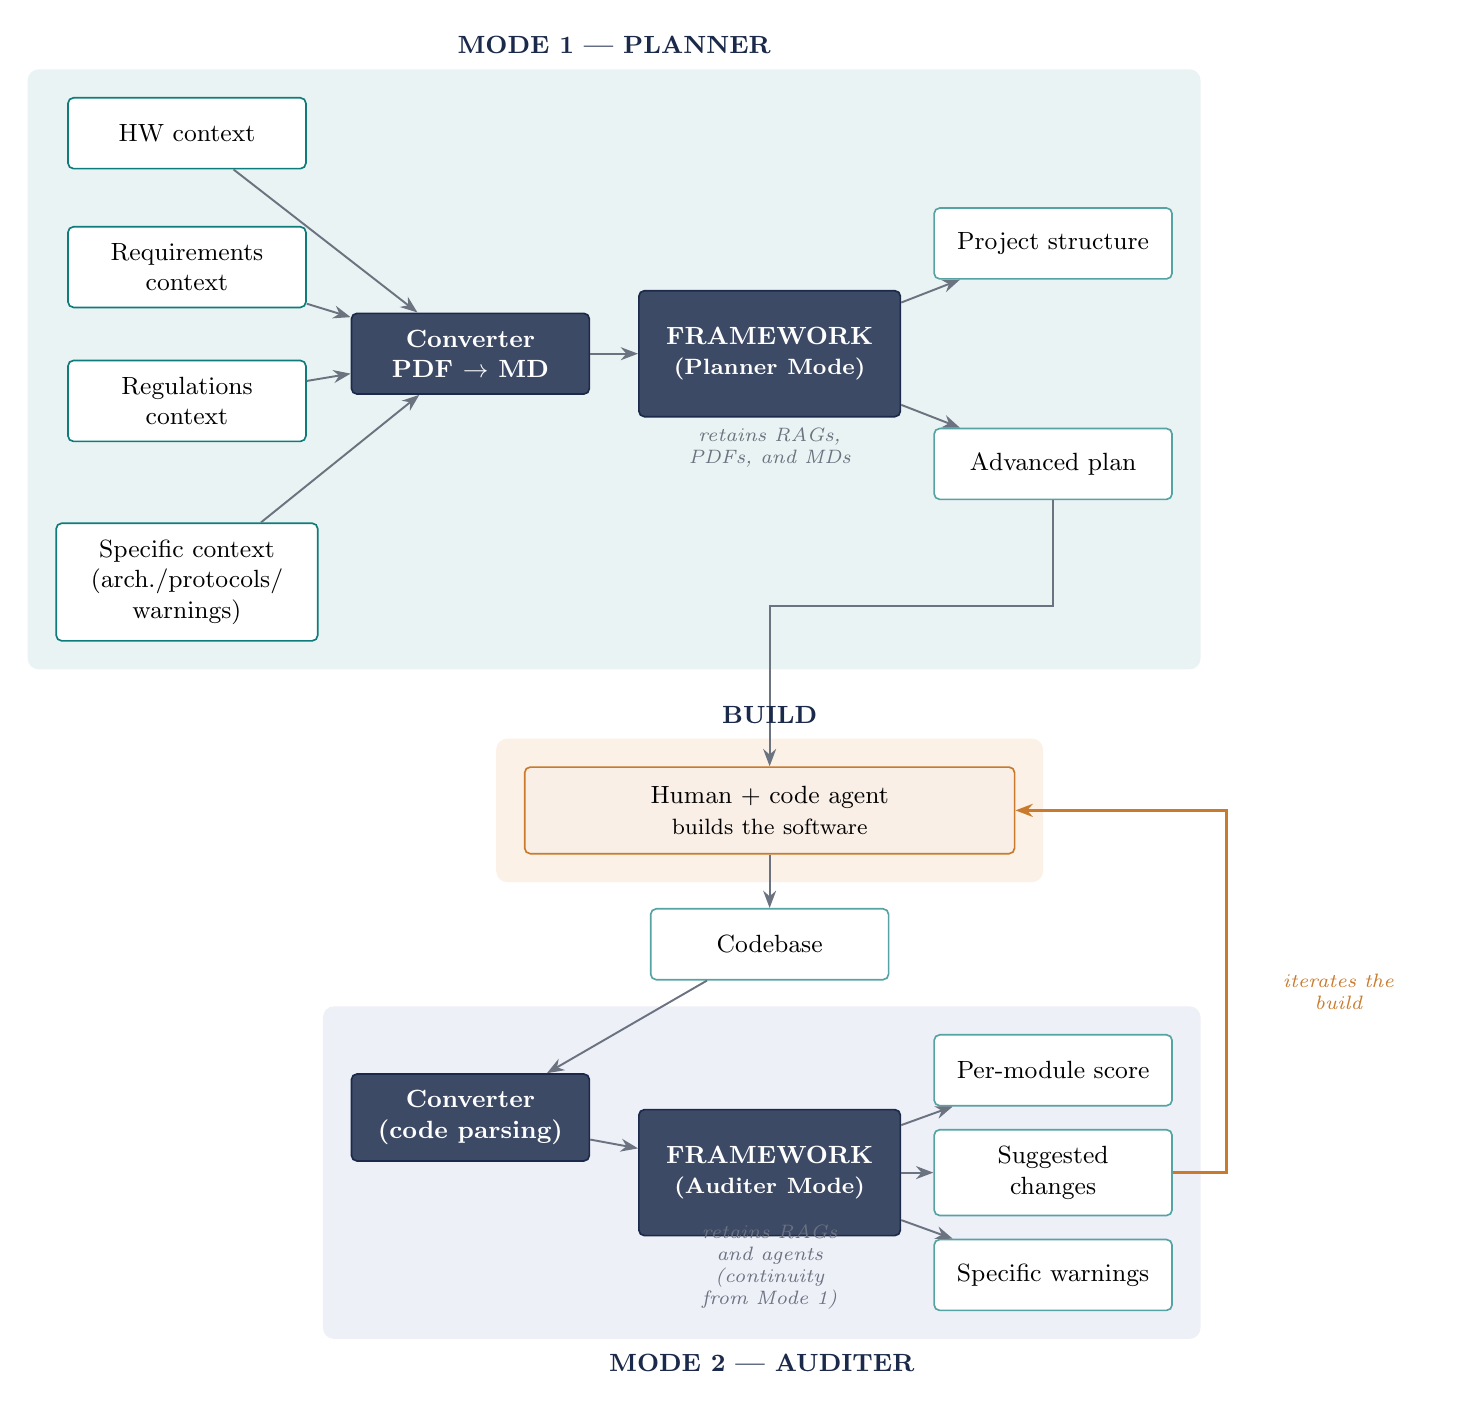
\begin{tikzpicture}[
  font=\small,
  box/.style={draw, rounded corners=2pt, align=center, minimum height=0.9cm, inner sep=6pt, line width=0.6pt},
  input/.style={box, draw=accentTeal, fill=white, text width=2.6cm},
  proc/.style={box, draw=inkNavy, fill=inkNavy!85, text=white, text width=3.2cm, font=\small\bfseries},
  outbox/.style={box, draw=accentTeal!70, fill=white, text width=2.6cm},
  human/.style={box, draw=accentAmber, fill=accentAmber!12, text width=4.6cm, minimum height=1.1cm},
  note/.style={font=\scriptsize\itshape, text=softGray, align=center},
  arr/.style={-{Stealth[length=2.2mm]}, line width=0.7pt, color=softGray},
  stagebg/.style={rounded corners=4pt, line width=0pt},
  stagelabel/.style={font=\bfseries\small, text=inkNavy}
]

% ---------- COLUMN 1: PLANNER MODE ----------
\node[input] (hw) at (0,8.0) {HW context};
\node[input] (req) at (0,6.3) {Requirements context};
\node[input] (norm) at (0,4.6) {Regulations context};
\node[input, text width=2.9cm] (esp) at (0,2.3) {Specific context\\(arch./protocols/\\warnings)};

\node[proc, text width=2.6cm] (conv1) at (3.6,5.2) {Converter\\PDF \(\to\) MD};
\node[proc, text width=2.9cm, minimum height=1.6cm] (fw1) at (7.4,5.2) {FRAMEWORK\\\footnotesize (Planner Mode)};
\node[note, text width=2.9cm] at (7.4,4.0) {retains RAGs,\\PDFs, and MDs};

\node[outbox] (struct) at (11.0,6.6) {Project structure};
\node[outbox] (plan) at (11.0,3.8) {Advanced plan};

\draw[arr] (hw) -- (conv1);
\draw[arr] (req) -- (conv1);
\draw[arr] (norm) -- (conv1);
\draw[arr] (esp) -- (conv1);
\draw[arr] (conv1) -- (fw1);
\draw[arr] (fw1) -- (struct);
\draw[arr] (fw1) -- (plan);

\begin{scope}[on background layer]
\node[stagebg, fill=bgPlanner, fit=(hw)(req)(norm)(esp)(conv1)(fw1)(struct)(plan), inner sep=10pt] (stage1) {};
\end{scope}
\node[stagelabel] at (stage1.north) [above, yshift=2pt] {MODE 1 --- PLANNER};

% ---------- STAGE 2: HUMAN + AGENT ----------
\node[human, text width=5.8cm] (build) at (7.4,-0.6) {Human + code agent\\\footnotesize builds the software};
\node[outbox, fill=white] (code) at (7.4,-2.3) {Codebase};

% Advanced plan -> Build (right-angle route, avoiding text overlap)
\draw[arr] (plan.south) -- (11.0,2.0) -- (7.4,2.0) -- (build.north);
\draw[arr] (build) -- (code);

\begin{scope}[on background layer]
\node[stagebg, fill=bgBuild, fit=(build), inner sep=10pt] (stage2) {};
\end{scope}
\node[stagelabel] at (stage2.north) [above, yshift=2pt] {BUILD};

% ---------- COLUMN 3: AUDITER MODE ----------
\node[proc, text width=2.6cm] (conv2) at (3.6,-4.5) {Converter\\(code parsing)};
\node[proc, text width=2.9cm, minimum height=1.6cm] (fw2) at (7.4,-5.2) {FRAMEWORK\\\footnotesize (Auditer Mode)};
\node[note, text width=3.1cm] at (7.4,-6.4) {retains RAGs\\and agents\\(continuity from Mode 1)};

\node[outbox] (score) at (11.0,-3.9) {Per-module score};
\node[outbox] (changes) at (11.0,-5.2) {Suggested changes};
\node[outbox] (warn) at (11.0,-6.5) {Specific warnings};

\draw[arr] (code) -- (conv2);
\draw[arr] (conv2) -- (fw2);
\draw[arr] (fw2) -- (score);
\draw[arr] (fw2) -- (changes);
\draw[arr] (fw2) -- (warn);

\begin{scope}[on background layer]
\node[stagebg, fill=bgAudit, fit=(conv2)(fw2)(score)(changes)(warn), inner sep=10pt] (stage3) {};
\end{scope}
\node[stagelabel] at (stage3.south) [below, yshift=-2pt] {MODE 2 --- AUDITER};

% ---------- FEEDBACK LOOP (outer route, no crossings) ----------
\draw[arr, color=accentAmber, line width=1pt] (changes.east) -- (13.2,-5.2) -- (13.2,-0.6) -- (build.east);
\node[note, text width=2.6cm, text=accentAmber] at (13.2,-2.9) [right] {iterates the\\build};

\end{tikzpicture}%
}
\caption{\small Conceptual flow: context flows from the Planner to the Build stage and from there to the Auditor, without the agent ever touching production code directly. Suggested changes and warnings feed back into the build cycle.}
\end{figure}

\subsection{Reading the diagram}

\begin{itemize}
  \item \textbf{Mode 1} normalizes four distinct context sources (hardware, requirements, regulations, specific context) through a single PDF\,\(\to\)\,MD converter, so the Framework always works on homogeneous text. The output is not code: it is a project structure and an advanced plan, and the Framework retains the source material as a persistent knowledge base.
  \item \textbf{The build stage} is deliberately human. The advanced plan and the retained context feed the developer and their code agent of choice, but the implementation decisions remain in human hands.
  \item \textbf{Mode 2} receives the resulting code (via a dedicated converter geared toward code parsing) and the same advanced plan. The Framework in this mode does not start from scratch: it retains the RAGs and agents from Mode 1, so it can audit the code against the original documentation, not just against the plan.
\end{itemize}

% ================= DESIGN PRINCIPLES =================
\section{Design principles}

\begin{ideabox}{Self-hosted by default}
LLM models running on local hardware. No hardware datasheet, internal regulation, or line of code needs to leave your own infrastructure for the system to work.
\end{ideabox}

\vspace{0.4em}

\begin{ideabox}{The agent plans, the human builds}
Separating plan generation from code generation reduces the hallucination surface where it hurts most: architectural decisions. The code is still written by whoever holds the judgment and final responsibility.
\end{ideabox}

\vspace{0.4em}

\begin{ideabox}{Scoped planning, not generic templates}
The advanced plan does not come from the model's general knowledge: it comes from what the ingested documentation actually says. That makes it narrower, but also more reliable and easier to justify in a real audit.
\end{ideabox}

\vspace{0.4em}

\begin{ideabox}{Audit with memory, not blind audit}
By retaining RAGs and agents across modes, the auditor evaluates the code against the same source of truth that generated the plan --- not against a new, potentially different interpretation of the same problem.
\end{ideabox}

% ================= USE CASES =================
\section{Where this idea fits}

\begin{itemize}
  \item \textbf{Firmware or embedded systems} teams working with manufacturer datasheets and safety regulations (industrial, automotive, medical) who cannot upload those documents to a cloud LLM.
  \item Organizations with \textbf{data sovereignty requirements} that already have, or are willing to invest in, local compute for model inference.
  \item Projects where the \textbf{cost of a regulatory misinterpretation} is high, and where having a plan traceable to the source documentation has value in itself, beyond development speed.
\end{itemize}

% ================= CLOSING =================
\section{In one sentence}

\begin{center}
\begin{tcolorbox}[
  enhanced, colback=inkNavy, colframe=inkNavy,
  coltext=white, width=0.9\textwidth, halign=center,
  arc=3pt, boxrule=0pt
]
\large\itshape ``An orchestrator that separates thinking, building, and verifying --- one that never assumes what the documentation doesn't say, and never leaves the hardware it runs on.''
\end{tcolorbox}
\end{center}

\end{document}
